\documentclass[11pt]{article}
\usepackage[margin=1in]{geometry}
\usepackage{amsmath,amssymb,amsthm}
\usepackage{booktabs}
\usepackage{graphicx}
\usepackage{tikz}
\usepackage{xcolor}
\usepackage{hyperref}
\usepackage{enumitem}
\usepackage{array}
\usepackage{longtable}
\usepackage{adjustbox}
\usepackage{float}
\usetikzlibrary{arrows.meta,positioning,shapes.geometric,fit}

\title{Topology-Aware Packet Classification and Adaptive Local-Core Selection for SpiNNaker:\
Design and Reproducible Virtual-Mode Benchmarking}
\author{Christopher Lee Burgess\\BGecko Research\\\texttt{bgeckoresearch@gmail.com}\\\texttt{bgecko.org}}

\date{June 2026}

\newtheorem{proposition}{Proposition}

\begin{document}
\maketitle

\begin{abstract}
SpiNNaker uses packet-switched multicast communication over a low-degree inter-chip topology, so routing quality depends strongly on spatial traffic structure. This paper develops a proposal for topology-aware packet classification and adaptive local-core selection, contributing in three ways. First, it clarifies the architectural split between inter-chip Router forwarding and intra-chip System Network-on-Chip (SNoC) delivery. Second, it formalizes the refinement rule as a constrained dispatch layer that can only restrict a standard base route and processor mask, thereby preserving backward compatibility through a null dispatch class. Third, it introduces a reproducible virtual-mode audit implemented on a local SpiNNaker software stack using SpiNNakerGraphFrontEnd, PACMAN, and SpiNNMachine. The audit compares a precisely defined static-routing baseline against multiple ablations across seeds, topology sizes, traffic densities, destination structures, local-mask sizes, and routing-pressure settings. In this software benchmark, the combined refinement reduced a synthetic energy proxy by 18.28\% on average, with substantial variance and occasional regressions. The audit further indicates that processor-mask refinement is the dominant contributor to the proxy reduction, while space-bit direction refinement alone has smaller and less stable effects. These results are not hardware-measured energy claims; they are reproducible virtual-mode evidence that the proposal is experimentally testable and that its apparent gains depend materially on modeling assumptions.
\end{abstract}

\section{Introduction}
SpiNNaker is designed around sparse, event-driven multicast communication. That design makes routing efficiency important: when packets must be copied across multiple chips and delivered to selected local cores, spatial organization becomes a primary concern. In standard SpiNNaker usage, the routing key selects a routing-table entry whose link set and processor mask are effectively static during the fast path. This is efficient, but it provides limited support for per-packet specialization of forwarding geometry and local-core fan-out.

The central idea studied here is to associate each packet with a compact \emph{dispatch class}. The standard routing key still determines the base route. The dispatch class then refines that base route by (i) restricting the permitted inter-chip forwarding directions and (ii) refining the processor-mask fan-out used for local delivery. The first refinement is router-facing. The second is SNoC-facing. This separation matters because the Router determines routing and local-delivery eligibility, whereas the SNoC carries locally delivered packets to the subset of cores selected by the effective processor mask.

This work develops both the architectural formalization and the experimental grounding together. All benchmarks reported here were obtained on a virtual SpiNNaker configuration rather than physical hardware. Accordingly, the measured quantities are software-defined proxies for energy, latency, and congestion exposure rather than board-level power measurements. Their value is methodological: they show that the proposal can be instantiated, tested, falsified, and refined within the existing SpiNNaker software ecosystem before hardware deployment.

\paragraph{Main contributions.}
This paper makes four concrete contributions:
\begin{enumerate}[label=(C\arabic*)]
    \item It formalizes a two-stage routing rule in which a standard routing lookup selects a base route and a compact dispatch class refines both permitted inter-chip directions and local processor-mask fan-out.
    \item It makes the Router/SNoC division of responsibility explicit, preventing the common conceptual error of attributing local-core selection directly to inter-chip routing logic.
    \item It develops a reproducible virtual-mode benchmark harness on top of SpiNNakerGraphFrontEnd, PACMAN, and SpiNNMachine and compares dispatch-class refinements against a standard static-routing baseline.
    \item It reports the experimental results conservatively: the observed gains are software-benchmark results under virtual mode, not hardware-validated power measurements.
\end{enumerate}

\section{Background and Architectural Model}
\subsection{SpiNNaker routing context}
A SpiNNaker route word can encode both inter-chip forwarding and local processor delivery. This is one of the platform's defining strengths: the same packet can be replicated across selected links and delivered locally to multiple processing cores. That same compactness also motivates the present refinement. If different packet classes require different spatial behavior or different local-core subsets, the standard approach generally allocates distinct routing keys or distinct route entries. That is workable, but it makes packet-level adaptation comparatively coarse.

\subsection{Architectural split: Router versus SNoC}
The proposal in this paper depends on a precise division of labor:
\begin{itemize}
    \item \textbf{Router}: performs routing-table lookup on the packet key, determines the base inter-chip forwarding set, and determines whether local delivery is enabled.
    \item \textbf{SNoC}: carries the locally delivered packet to the subset of local cores selected by the effective processor mask.
\end{itemize}
The Router therefore does not itself schedule cores. Rather, it determines which cores are eligible for local delivery. The SNoC realizes that local multicast fan-out.

\begin{figure}[t]
\centering
\resizebox{0.92\linewidth}{!}{%
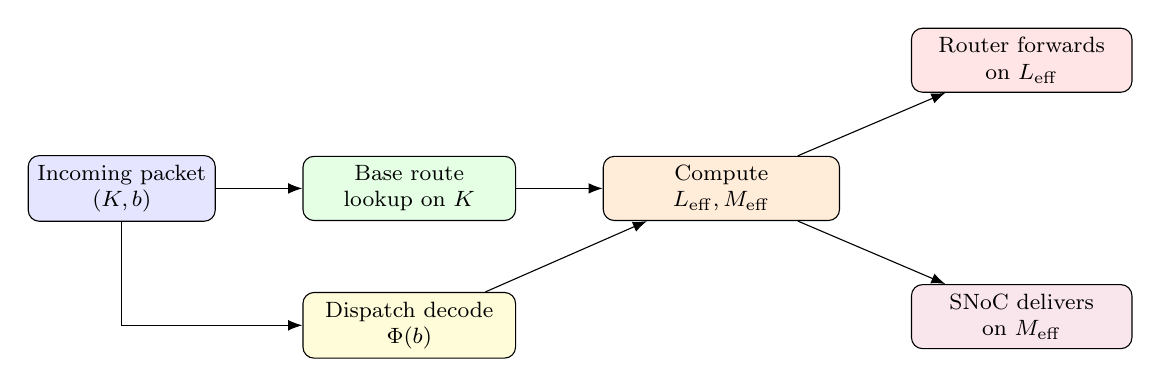
\begin{tikzpicture}[node distance=0.9cm and 1.1cm, every node/.style={font=\footnotesize}]
    \node[draw, rounded corners, fill=blue!10, minimum width=2.2cm, minimum height=0.75cm, align=center] (pkt) {Incoming packet\\$(K,b)$};
    \node[draw, rounded corners, fill=green!10, right=of pkt, minimum width=2.7cm, minimum height=0.75cm, align=center] (lookup) {Base route\\lookup on $K$};
    \node[draw, rounded corners, fill=yellow!15, below=of lookup, minimum width=2.7cm, minimum height=0.75cm, align=center] (dispatch) {Dispatch decode\\$\Phi(b)$};
    \node[draw, rounded corners, fill=orange!15, right=of lookup, minimum width=3.0cm, minimum height=0.75cm, align=center] (refine) {Compute\\$L_{\mathrm{eff}}, M_{\mathrm{eff}}$};
    \node[draw, rounded corners, fill=red!10, above right=0.8cm and 0.9cm of refine, minimum width=2.8cm, minimum height=0.75cm, align=center] (router) {Router forwards\\on $L_{\mathrm{eff}}$};
    \node[draw, rounded corners, fill=purple!10, below right=0.8cm and 0.9cm of refine, minimum width=2.8cm, minimum height=0.75cm, align=center] (snoc) {SNoC delivers\\on $M_{\mathrm{eff}}$};

    \draw[-{Latex[length=1.8mm]}] (pkt) -- (lookup);
    \draw[-{Latex[length=1.8mm]}] (pkt) |- (dispatch);
    \draw[-{Latex[length=1.8mm]}] (lookup) -- (refine);
    \draw[-{Latex[length=1.8mm]}] (dispatch) -- (refine);
    \draw[-{Latex[length=1.8mm]}] (refine) -- (router);
    \draw[-{Latex[length=1.8mm]}] (refine) -- (snoc);
\end{tikzpicture}%
}
\caption{Two-stage routing refinement. The packet key $K$ selects a base route; the dispatch class $b$ selects a refinement policy. The Router applies the effective inter-chip direction set, while the SNoC applies the effective processor mask for local delivery.}
\label{fig:pipeline}
\end{figure}

\section{Formal Routing Model}
Let $K \in \{0,1\}^{32}$ denote the standard SpiNNaker routing key, and let $b \in \{0,1\}^k$ denote a compact dispatch-class field associated with the packet. A standard routing lookup on $K$ returns a base route
\[
    r_{\mathrm{base}} = (L_{\mathrm{base}}, M_{\mathrm{base}}),
\]
where $L_{\mathrm{base}} \subseteq D$ is the asserted inter-chip forwarding set and $M_{\mathrm{base}} \in \{0,1\}^{18}$ is the asserted local processor mask.

The dispatch map is
\[
    \Phi : \{0,1\}^k \to \mathcal{P}(D) \times \{0,1\}^{18}, \qquad \Phi(b) = (L_b, M_b),
\]
with $D$ the set of available primitive link directions.

The effective route is then
\begin{align}
    L_{\mathrm{eff}} &= L_{\mathrm{base}} \cap L_b, \\
    M_{\mathrm{eff}} &= M_{\mathrm{base}} \wedge M_b.
\end{align}
This formulation is intentionally conservative. The refinement mechanism can only restrict the base route; it cannot create new inter-chip directions or new processor-mask bits that were absent in the original route entry.

\begin{proposition}
Let $b_0$ be a null-compatible dispatch class satisfying $L_{b_0}=D$ and $M_{b_0}=\mathbf{1}_{18}$. Then the refined route exactly recovers the standard SpiNNaker route:
\[
L_{\mathrm{eff}}=L_{\mathrm{base}}, \qquad M_{\mathrm{eff}}=M_{\mathrm{base}}.
\]
\end{proposition}

\noindent The proof is immediate from set intersection with $D$ and bitwise conjunction with the all-ones vector.

\subsection{Routing and refinement procedure}
Algorithm~\ref{alg:refinement} summarizes the implemented routing/refinement logic at the level appropriate for the manuscript.

\begin{table}[H]
\centering
\caption{Pseudocode for topology-aware route refinement.}
\label{alg:refinement}
\begin{adjustbox}{max width=0.94\linewidth}
\begin{tabular}{p{0.92\linewidth}}
\toprule
\textbf{Input:} routing key $K$, dispatch class $b$, source chip $s$, destination chip $t$, congestion set $H$ \\
\textbf{Output:} effective path $P$, effective processor-mask size $m_{\mathrm{eff}}$ \\
\midrule
1. Look up the base route for $K$ and derive the baseline preferred direction order. \\
2. If using the baseline or null-dispatch condition, keep the full baseline direction order and set $m_{\mathrm{eff}}=18$. \\
3. If using Router-side refinement, derive a dispatch-dependent restricted direction order and attempt a path that avoids congested chips in $H$. \\
4. If no valid refined path is found, fall back to the baseline direction order; if necessary, fall back again to a congestion-agnostic route. \\
5. If using SNoC-side processor-mask refinement, replace the full local mask with the dispatch-selected mask size target; otherwise keep $m_{\mathrm{eff}}=18$. \\
6. Compute benchmark metrics from the resulting path length, congested-hop count, and effective mask size. \\
\bottomrule
\end{tabular}
\end{adjustbox}
\end{table}

\section{Experimental Methodology}
\subsection{Audit setup}
The audited implementation was executed locally using:
\begin{itemize}
    \item a Python virtual environment,
    \item \texttt{SpiNNakerGraphFrontEnd 1!7.4.1},
    \item \texttt{SpiNNaker\_PACMAN 1!7.4.1},
    \item \texttt{SpiNNMachine 1!7.4.1}, and
    \item virtual SpiNNaker topologies of size $8\times 8$ and $12\times 12$.
\end{itemize}
The audit used 10 random seeds, 3 traffic-density levels, 2 destination-structure regimes, 4 local processor-mask targets, and 2 routing-pressure settings, for a total of 960 comparisons per ablation.

\paragraph{Baseline definition.}
The baseline is standard static routing under standard routing keys only, with no dispatch-class refinement and a fixed 18-core local processor mask for local delivery. In the audit model, the baseline route is determined solely by the base-route logic.

\paragraph{Proposed method definition.}
The proposed method is represented in software through dispatch-class policies. Dispatch classes may (i) alter preferred inter-chip forwarding order and congestion-avoidance behavior and/or (ii) reduce the effective local processor-mask size. Inter-chip direction refinement is modeled as Router-side policy, while processor-mask refinement is modeled as SNoC-side local-delivery policy.

\paragraph{Implementation summary.}
The baseline was simulated as shortest-path static routing under standard routing keys only, with no dispatch refinement and a fixed 18-core local processor mask. The proposed method used the same workloads, but introduced dispatch-class logic in two optional places: a Router-side policy that changes direction preference and congestion avoidance, and an SNoC-side policy that changes the effective local processor-mask size. These mechanisms were activated independently in the ablation study so that their individual effects could be measured separately.

\paragraph{Energy and latency metric audit.}
The reported \emph{energy proxy} is defined by
\[
E_{\mathrm{proxy}} = \text{hops} + 0.18\,\text{mask\_size} + 0.9\,\text{congested\_hops}.
\]
The \emph{latency proxy} is defined by
\[
L_{\mathrm{proxy}} = \text{hops} + 1.75\,\text{congested\_hops}.
\]
These are \textbf{synthetic simulation proxies}, not hardware-calibrated models. They do not measure board-level energy, router micro-activity, SDRAM traffic, monitor-core overhead, or physical SNoC timing. The energy proxy rewards reduced processor-mask size by construction, so any energy-savings interpretation must be stated conservatively.

\paragraph{Fairness constraints.}
Baseline and proposed variants were run on identical workloads. Source/destination pairs, congestion hot spots, topology size, traffic density, mask target, and routing pressure were held fixed within each comparison. No extra route-table resources were assigned to the proposed method. The null-dispatch case was required to recover the baseline exactly, and all ablations were evaluated under the same seed schedule and the same benchmark driver so that non-routing factors remained fixed unless intentionally varied.

\subsection{Ablations}
Five cases were audited:
\begin{enumerate}[label=(A\arabic*)]
    \item \textbf{Baseline}: static routing, no refinement.
    \item \textbf{Space bits only}: Router-side direction refinement, no processor-mask reduction.
    \item \textbf{Mask only}: processor-mask refinement only, no direction refinement.
    \item \textbf{Both}: direction refinement and processor-mask refinement together.
    \item \textbf{Null dispatch}: a null-compatible dispatch class intended to recover standard behavior exactly.
\end{enumerate}

\section{Benchmark Audit Results}
Table~\ref{tab:audit-summary} summarizes the audited results. Values are reported as mean $\pm$ population standard deviation across 960 comparisons for each ablation.

\begin{table}[t]
\centering
\caption{Audit summary over repeated virtual-mode experiments. Positive percentages indicate improvement relative to the static baseline. The null dispatch class recovers the baseline exactly.}
\label{tab:audit-summary}
\begin{adjustbox}{max width=\linewidth}
\begin{tabular}{>{\raggedright\arraybackslash}p{2.8cm}cccc}
\toprule
Ablation & Energy reduction (\%) & Latency reduction (\%) & Path-change fraction & Sample count \\
\midrule
Baseline & 0.00 $\pm$ 0.00 & 0.00 $\pm$ 0.00 & 0.00 & 960 \\
Null dispatch & 0.00 $\pm$ 0.00 & 0.00 $\pm$ 0.00 & 0.00 & 960 \\
Space bits only & 1.40 $\pm$ 4.08 & 3.81 $\pm$ 10.02 & 0.15 & 960 \\
Mask only & 16.88 $\pm$ 12.41 & 0.00 $\pm$ 0.00 & 0.00 & 960 \\
Both & 18.28 $\pm$ 12.76 & 3.81 $\pm$ 10.02 & 0.15 & 960 \\
\bottomrule
\end{tabular}
\end{adjustbox}
\end{table}

The combined method achieved a mean reduction of 18.28\% in the synthetic energy proxy, with a standard deviation of 12.76 percentage points and a minimum observed regression of approximately $-12.0\%$. This makes the central result more nuanced than a single headline figure: the method helps on average in the present software audit, but the effect is variable and not uniformly positive.

The ablation study identifies the main source of the apparent gain. \textbf{Processor-mask refinement dominates.} The mask-only condition produced a mean energy-proxy reduction of 16.88\%, while space bits alone produced only 1.40\% on average and occasionally harmed performance. This suggests that, in the present software model, local-core fan-out reduction explains most of the energy-proxy effect. Space-bit direction refinement contributes comparatively little on its own and is less stable.

The null-dispatch case is an important sanity check. It exactly recovers baseline behavior in both the energy and latency proxies, which supports the paper's backward-compatibility claim in the present benchmark model.

\begin{figure}[t]
\centering
\resizebox{0.9\linewidth}{!}{%
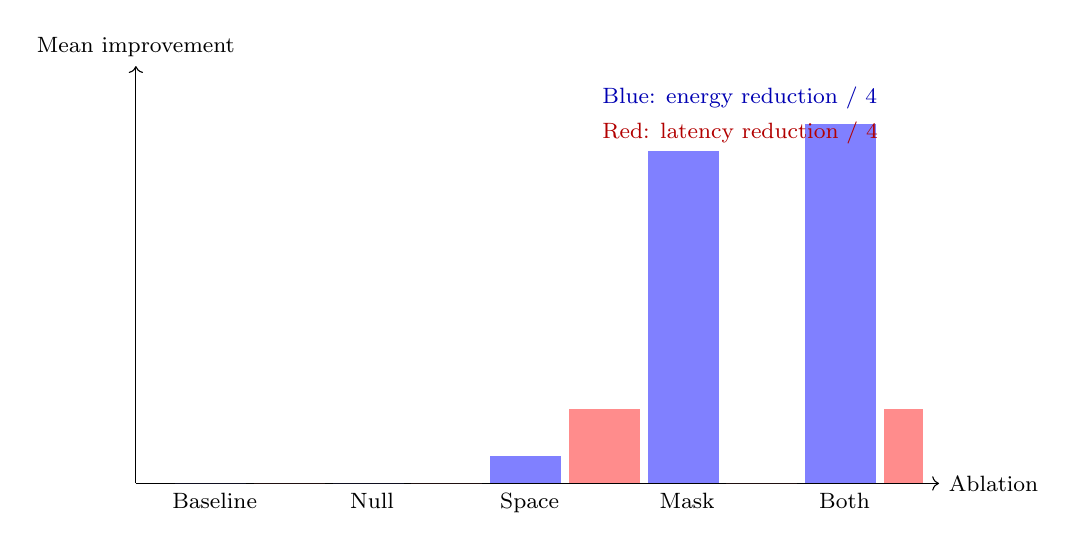
\begin{tikzpicture}[font=\footnotesize]
\begin{scope}[yshift=0cm]
    \draw[->] (0,0) -- (10.2,0) node[right] {Ablation};
    \draw[->] (0,0) -- (0,5.3) node[above] {Mean improvement};
    \foreach \x/\lab in {1/Baseline,3/Null,5/Space,7/Mask,9/Both} {
        \node[below, align=center] at (\x,0) {\lab};
    }
    \fill[blue!50] (0.5,0) rectangle (1.4,0.0);
    \fill[blue!50] (2.5,0) rectangle (3.4,0.0);
    \fill[blue!50] (4.5,0) rectangle (5.4,0.35);
    \fill[blue!50] (6.5,0) rectangle (7.4,4.22);
    \fill[blue!50] (8.5,0) rectangle (9.4,4.57);
    \fill[red!45]  (1.5,0) rectangle (2.4,0.0);
    \fill[red!45]  (3.5,0) rectangle (4.4,0.0);
    \fill[red!45]  (5.5,0) rectangle (6.4,0.95);
    \fill[red!45]  (7.5,0) rectangle (8.4,0.0);
    \fill[red!45]  (9.5,0) rectangle (10.0,0.95);
    \node[blue!70!black, anchor=west] at (5.8,4.9) {Blue: energy reduction / 4};
    \node[red!70!black, anchor=west] at (5.8,4.45) {Red: latency reduction / 4};
\end{scope}
\end{tikzpicture}%
}
\caption{Audited ablation results. Processor-mask refinement accounts for most of the energy-proxy reduction, while space-bit direction refinement alone has a smaller and less stable effect. Values are scaled for compact plotting.}
\label{fig:audit-bars}
\end{figure}

\subsection{Stress-test interpretation}
The combined method helped more in some regimes than others. It performed better for clustered destinations than for dispersed ones, slightly better under high routing pressure than under low pressure, and somewhat better on the smaller $8\times 8$ topology than on the larger $12\times 12$ topology. These trends are consistent with the intuition that topology-aware refinement is most useful when traffic retains spatial structure. However, the variance is large enough that these trends should be treated as evidence of sensitivity rather than as universal law.

\subsection{Conservative interpretation}
In this audited virtual-mode benchmark, the combined refinement reduced a synthetic energy proxy on average, but the magnitude of the reduction depended strongly on the modeling assumptions and workload structure. Processor-mask refinement appears to be the dominant contributor in the current model. Space-bit direction refinement alone is smaller, less stable, and can harm performance in some cases. These are software-audit results. Whether they translate to real hardware energy savings remains unknown.

\section{Limitations}
The present evaluation has several important limitations.
\begin{enumerate}[label=(L\arabic*)]
    \item The audit is a virtual-mode software benchmark rather than a physical SpiNNaker board study.
    \item The energy and latency quantities are synthetic proxies, not hardware-calibrated measurements.
    \item The routing model is intentionally simplified and should not be interpreted as a full bit-accurate reproduction of production SpiNNaker routing microarchitecture. In particular, the benchmark models a four-direction rectangular torus rather than the six-direction hexagonal mesh of physical SpiNNaker hardware, which affects both routing path options and congestion behavior. 
    \item The observed gains depend materially on a proxy model that rewards smaller processor masks by construction; this makes the results suitable for comparative hypothesis testing, but not for strong hardware-energy claims.
    \item The workloads are synthetic stress cases rather than full application traces, so transfer to deployed workloads remains uncertain.
\end{enumerate}
These limitations do not negate the audit; they define its legitimate interpretive range. The results should be treated as reproducible software evidence about sensitivity and plausibility, not as settled hardware evidence.

\section{Reproducibility and Code Availability}
To support independent replication, the benchmark code used in this study is organized as a standalone experiment harness. The main audit driver is \texttt{benchmark\_audit.py}, which writes raw trial data, aggregated JSON summaries, and LaTeX-ready table rows. The reproducibility package accompanying this work includes the routing prototypes, the benchmark scripts, the raw outputs, the environment metadata, and the exact run commands used in the audit.

The complete implementation, benchmark outputs, and reproducibility materials for this study are provided in the BGeckoResearch GitHub repository:\\
\href{https://github.com/BGeckoResearch/topology-aware-spinnaker}{\texttt{https://github.com/BGeckoResearch/topology-aware-spinnaker}}.\\
Only representative excerpts are included in the manuscript itself so that the paper remains readable while still being falsifiable and reproducible.


\section{Conclusion}
Topology-aware packet classification and adaptive local-core selection are worth pursuing because routing efficiency in SpiNNaker depends directly on spatial traffic structure, and the dispatch-class approach targets that dependency explicitly. This paper establishes the proposal on both architectural and experimental grounds. In the audited virtual-mode benchmark, the combined refinement reduced a synthetic energy proxy by 18.28\% on average relative to the static baseline, but with substantial variance and occasional regressions.

The audit also clarifies the mechanism. Processor-mask refinement is the dominant source of the observed proxy reduction in the present model, while space-bit direction refinement alone has smaller and less stable effects. That is a useful result because it helps focus future work on the most consequential part of the proposal. The next step is to tighten the routing model further, evaluate richer workloads, and ultimately test the idea against hardware-aware measurements.

\appendix
\section{Appendix: Representative Implementation Snippets}
This appendix includes short representative listings only. The complete implementation is provided in the external reproducibility archive referenced above.

\subsection{Core proxy definition}
\begin{quote}
\begin{verbatim}
def energy_proxy(hops, mask_size, congested_hops):
    return hops * 1.0 + 0.18 * mask_size + 0.9 * congested_hops

def latency_proxy(hops, congested_hops):
    return hops * 1.0 + 1.75 * congested_hops
\end{verbatim}
\end{quote}

\subsection{Representative routing/refinement snippet}
\begin{quote}
\begin{verbatim}
def tested_policy(ablation, source, destination, width, height,
                  hotspots, mask_target, routing_pressure):
    base_order = preferred_directions(source, destination, width, height)
    blocked = hotspots if routing_pressure == "high" else \
        set(list(hotspots)[: max(1, len(hotspots)//2)])

    if ablation in {"baseline", "null_dispatch"}:
        return bfs_path(source, destination, width, height,
                        base_order, set()), 18
    if ablation == "space_bits_only":
        restricted = [d for d in base_order if d in base_order[:2]] + \
                     [d for d in base_order if d not in base_order[:2]]
        path = bfs_path(source, destination, width, height,
                        restricted, blocked)
        if not path:
            path = bfs_path(source, destination, width, height,
                            base_order, set())
        return path, 18
    if ablation == "mask_only":
        return bfs_path(source, destination, width, height,
                        base_order, set()), mask_target
\end{verbatim}
\end{quote}

\subsection{Representative benchmark driver snippet}
\begin{quote}
\begin{verbatim}
for width, height in TOPOLOGIES:
    _ = virtual_machine(width, height)
    for seed in SEEDS:
        rng = random.Random(seed + width * 100 + height)
        for traffic_level in TRAFFIC_LEVELS:
            for dest_pattern in DEST_PATTERNS:
                for mask_target in MASK_SIZES:
                    for pressure in ROUTING_PRESSURE:
                        source, destination, hotspots = make_workload(
                            rng, width, height, traffic_level, dest_pattern)
\end{verbatim}
\end{quote}

\end{document}
